\documentclass{article}
\usepackage[utf8]{inputenc}
\usepackage{graphicx}
\usepackage{amsmath}
\usepackage{amssymb}
\usepackage{hyperref}
\usepackage{natbib}
\usepackage{url}

\title{Revue de littérature sur les biais dans les algorithmes d’intelligence artificielle et dans les données
}
\author{GOUCEM Thinhinane, EL-OUESLATI Tasnime , Fikri-Kassim Ibrahim }
\date{Novembre 2025}
\begin{document}

\maketitle


La généralisation de l’utilisation de l’intelligence artificielle dans des domaines de la vie publique est un phénomène qui suscite l’inquiétude de par son enjeu critique. Et pour cause: une ia peut désormais décider du sort d’un individu: va t’il obtenir ce poste tant désiré? Ce crédit dont il a tant besoin? Ce traitement qui pourrait le sauver? Ou est ce que l’ia le condamnera injustement, mimant voir amplifiant les inégalités existantes. Car en effet, l’on a pu observer que les injustices sociales se reproduisaient dans les décisions ou recommandations que l’ia produisait, à cause de biais qu’elle aurait appris. Il est alors legitime de se demander comment les biais intégrés dans les données et les algorithmes d’IA influencent-ils les décisions automatisées dans différents domaines, et quelles solutions sont proposées pour les atténuer? 

De nombreux articles ont tenté de répondre à cette question et nous allons en analyser quelque uns. Ces articles ont tout d’abord été sélectionnés pour leur rigueur scientifique mais aussi leur portée et pluridisciplinarité, leur couverture des dernières avancées, leur clarté et visualité, leur réflexion à des solutions, leur indépendance, leur accessibilité, leur originalité et poids dans le domaine et leur angle d’approche. Nous avons sélectionné un article général\citep{ageneral2023} qui apporte une vue d’ensemble du sujet et en couvre les principaux aspects, un article théorique\citep{BarocasSelbst2016}, un article technique\citep{Mitchell1980} et un article empirique\citep{BuolamwiniG18} pour l’illustration d’un cas concret.

Pour les trouver, nous avons utilisés les mots clefs suivants (trouvés suite a la lectures de plusieurs articles généraux sur le sujet ou proposés par des banques de donnée ou générés par ia (prompt: Donne moi des mots clefs a tapper pour trouver des articles sur le sujet : «…» , certains mots clefs générés étaient très puissants mais d’autres pas assez inscris dan le sujet comme fairness contraints, reweighting techniques… ) pour interroger des bases des données et moteurs de recherche scientifiques: dataset debiasing, representation learning bias, sampling bias correction,fairness-aware machine learning, algorithmic debiasing methods, counterfactual fairness, post-processing debiasing algorithm, adversarial debiasing, fair GAN,  biais algorithmes et données ia, bias ia Survey. Nous avons ainsi trouvé une quarantaine d’articles correspondant au sujet.
Nous commenceront par synthétiser chaque articles puis discuterons de leurs points communs,  leurs spécificités et leurs limites.





Notre premier article intitulé Algorithmes: biais, discrimination et équité\citep{ageneral2023} est publié par Telecom Paris en 2019 explique comment les biais peuvent apparaître et comment on peut essayer de les limiter. Les auteurs rappellent d’abord que les algorithmes apprennent à partir de données historiques. Si ces données reflètent des inégalités ou des choix passés, le modèle risque de reproduire les mêmes problèmes. Les biais peuvent avoir plusieurs origines: certains viennent des concepteurs qui ont parfois des préférences ou des idées préconçues; d’autres viennent des données, par exemple quand elles sont partielles ou déséquilibrées; enfin, certains biais sont liés aux objectifs choisis pour l’algorithme, par exemple quand on optimise uniquement la performance sans penser à l’équité. L’article propose aussi des solutions pour limiter ces biais. On peut, par exemple, ajuster les données pour que tous les groupes soient correctement représentés, ajouter des contraintes dans le modèle pour qu’il soit plus équitable, ou corriger les décisions après coup. Les auteurs précisent cependant qu’il n’existe pas de solution universelle. Pour Finir les auteurs soutiennent que l’équité ne se résume pas à un problème technique. Il faut aussi penser aux aspects sociaux et éthiques, et impliquer des régulateurs ou des institutions pour superviser l’utilisation de ces systèmes. Les biais peuvent apparaître à différents niveaux: dans les données, dans les choix de conception ou dans les objectifs que l’on fixe aux modèles.

Notre deuxième article, The Need for Biases in Learning Generalizations\citep{Mitchell1980} de Tom Mitchell, publié en 1980 est un texte fondamental en apprentissage automatique. Dans cet article, Mitchell introduit pour la première fois le concept de biais inductif, qui désigne l’ensemble des hypothèses qu’un algorithme utilise pour pouvoir généraliser à partir de données limitées. Selon lui, tout algorithme d’apprentissage doit nécessairement faire ces hypothèses: sans elles, il serait impossible de tirer des conclusions fiables à partir d’exemples.
L’article explique que ces biais peuvent prendre différentes formes selon le type de modèle ou les choix de conception: par exemple, un biais peut pousser un algorithme à privilégier des règles simples plutôt que des relations plus complexes, ou à limiter le type de relations qu’il peut apprendre. Il nous apprends donc qu’il existe un autre type de biais que ceux que l’on a vu et dont on parle le plus souvent et que ce biais n’est pas négatif en soi, et meme indispensable pour que l’apprentissage fonctionne. Cette article est une référence pour les scientifiques et sert de base aux travaux qui analysent les biais techniques et les biais sociaux dans les systèmes d’IA modernes. Il fait partis des publication les plus ancienne sur les biais dans l’IA.


Notre troisième article, Gender Shades\citep{BuolamwiniG18}, publié par Joy Buolamwini et Timnit Gebru en 2018, s’intéresse lui à un problème concret: la reconnaissance faciale commerciale et ses erreurs selon le genre et la couleur de peau. Les autrices ont remarqué que les systèmes disponibles sur le marché n’étaient pas aussi fiables pour tout le monde. Pour vérifier cela, elles ont testé plusieurs modèles de reconnaissance faciale sur un ensemble de photos de personnes aux genres et teints de peau variés. Le résultat est frappant: les algorithmes reconnaissent très bien les hommes à peau claire, mais ils se trompent beaucoup plus souvent pour les femmes à peau foncée. Les écarts sont plutôt importants et peuvent avoir des conséquences réelles, surtout si ces systèmes sont utilisés pour des décisions importantes comme l’accès à des services, la surveillance ou même l’emploi. Les auteures expliquent que ce problème vient surtout des données utilisées pour entraîner les modèles. Si les bases de données contiennent surtout des photos d’hommes à peau claire, le modèle apprend mieux à les reconnaître et fait moins bien pour les autres groupes. Enfin, Buolamwini et Gebru proposent des pistes pour améliorer les systèmes: diversifier les données d’entraînement, mesurer les performances selon différents groupes et ajuster les modèles pour réduire les écarts. Ce travail nous apprends que les algorithmes ne sont pas neutres et que des tests empiriques sont indispensables pour comprendre leurs limites.
\begin{figure}[h]
    \centering
    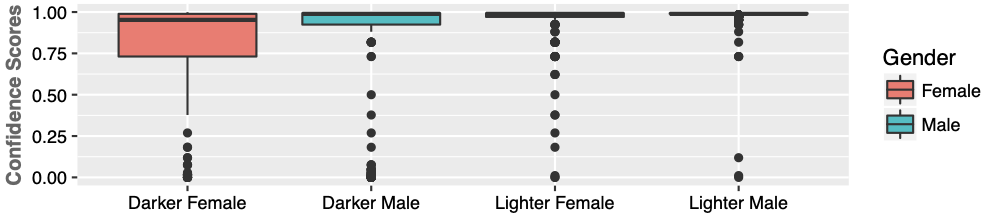
\includegraphics[width=0.8\linewidth]{image1.png}
    \caption{Distribution des scores de confiance en fonction du genre et de la teinte de peau}
    \label{fig:ma_image}
\end{figure}

Notre quatrième article est Big Data’s Disparate Impact\citep{BarocasSelbst2016} (Barocas \& Selbst, 2016). Dans cet article les auteurs montrent comment les systèmes d’analyse de données et les algorithmes peuvent produire des formes de discrimination même lorsqu’il n’y a pas d’ intention de discriminer. Leur analyse s’appuie sur le droit anti discriminatoire américain, qui interdit les pratiques professionnelles ayant un impact différentiel ( discrimination non intentionnelle) sur certains groupes protégés (par exemple selon le genre ou l’origine ethnique). Barocas et Selbst expliquent que les algorithmes posent un défi majeur à ce cadre légal. En effet, les systèmes de data-mining sont conçus pour trouver des corrélations efficaces pour prédire des comportements (réussite professionnelle, stabilité, productivité…). Si une caractéristique semble statistiquement utile, les entreprises peuvent la défendre comme une « nécessité commerciale », même si, indirectement, elle désavantage un groupe. Cela rend beaucoup plus difficile la contestation juridique, car les algorithmes donnent une apparence d’objectivité aux décisions. Un autre point clé de l’article est que les données historiques utilisées pour entraîner les modèles sont souvent marquées par des discriminations passées (comme des pratiques de recrutement biaisées). Ils montrent également que ces discriminations émergent à travers plusieurs mécanismes: l’usage de variables dites proxies, par exemple le code postal ou certains comportements d’achat qui reflètent indirectement des caractéristiques socio-économiques ou raciales; des bases de données déséquilibrées ou non représentatives; ou encore des phénomènes de rétroaction, comme dans les systèmes de police prédictive qui renforcent leurs propres présupposés en envoyant davantage de patrouilles dans les zones où les données signalent plus d’arrestations. Les algorithmes risquent alors de reproduire ces inégalités sans pour autant enfreindre explicitement la loi. Ces biais ne sont pas simples à corriger: modifier les données ou les résultats peut être perçu comme injuste, peu transparent, ou même illégal selon certaines interprétations juridiques. L’article se termine sur un constat: les outils d’aide à la décision sont capables de contourner les protections juridiques existantes. Cet article sera un déclencheur majeur de débats publics et d’ajustements industriels.

Nous avons jugé pertinent d'ajouter un article que nous avon lu mais que nous n'avons pas retenu dans la discussion. Il nous a donné des clefs pour comprendre le sujet et le couvrait de maniere assez intéressente puisque globale : Biais algorithmiques, enquete sur un danger réel. Cet article dresse tout d'abord un état de l'art de la question, il fournit donc un base necessaire puis alerte sur la menace sociétale que constitue les biais. Enfin il propose l'ensemble des solutions préconisées par les experts.  

Les quatre articles que nous avons présenté abordent tous la question des biais dans les algorithmes et dans les données, mais chacun le fait depuis un angle différent. On remarque d’abord que tous les textes reconnaissent que les systèmes d’IA ne sont jamais complètement neutres: ils reflètent soit la manière dont ils ont été construits, soit les données dont ils dépendent, soit les choix techniques effectués par leurs concepteurs. Le premier article, propose une vue d’ensemble et cherche surtout à clarifier les différents types de biais possibles. Il est très pédagogique par rapport aux autres et montre que les biais peuvent venir des données, des concepteurs ou des objectifs d’optimisation, et qu’il faut combiner plusieurs approches pour espérer les réduire. L’article Gender Shades incarne, lui, le passage à une démarche empirique et concrète. 

Contrairement au texte précédent, qui décrit les biais de manière théorique, ici les autrices démontrent précisément, chiffres à l’appui, comment un modèle peut discriminer selon le genre et la couleur de peau. Leur travail révèle une inégalité très nette entre différents groupes et montre que ces écarts ne sont pas de simples imperfections techniques mais bien des problèmes structurels liés aux jeux de données. Ce papier complète et illustre directement les concepts plus généraux décrits par Telecom Paris: il en est presque la preuve expérimentale. De son côté, Barocas \& Selbst ouvrent un autre champ: celui du droit et des conséquences sociales. Leur contribution est importante parce qu’elle montre que les biais algorithmiques ne posent pas seulement un problème de performance ou de qualité scientifique, mais aussi un problème de justice. Ils expliquent comment les algorithmes de big data peuvent produire un “impact différentiel”, c’est-à-dire des conséquences discriminatoires sur certains groupes, même sans intention malveillante. Ce texte est donc complémentaire des deux premiers: il met en lumière le décalage entre les réalités techniques de l’IA et les catégories juridiques traditionnelles, et il montre que la régulation n’est pas encore adaptée aux nouveaux risques posés par les modèles d’apprentissage.	Enfin, l’article de Tom Mitchell (1980) occupe une place à part. C’est le plus ancien du corpus, et il ne parle pas des biais au sens social ou éthique du terme. Il introduit plutôt le concept de «biais inductif», autrement dit les hypothèses préalables dont un algorithme a besoin pour apprendre. Ce biais n’est pas un problème, mais une condition nécessaire à l’apprentissage automatique. Ce texte donne un éclairage historique essentiel: il montre que la notion de “biais” a évolué au fil du temps. Au départ, il s’agissait d’un concept purement technique; aujourd’hui, il renvoie surtout à des questions d’équité. Cette évolution terminologique illustre bien la manière dont l’IA s’est progressivement rapprochée des enjeux sociaux.

En comparant ces articles, on observe donc un fil directeur: la compréhension des biais est passée d’un problème interne au fonctionnement des algorithmes (Mitchell), à une préoccupation socio-technique théorisée (Telecom Paris), puis à des démonstrations concrètes de discriminations produites par les modèles (Gender Shades), avant d’être analysée comme un défi juridique et politique (Barocas \& Selbst). Chacun met en avant un niveau différent du problème: le niveau technique, le niveau statistique, le niveau empirique et le niveau institutionnel.

On peut aussi noter quelques divergences. Mitchell considère le biais comme un élément indispensable et neutre, alors que les autres articles l’associent à un risque qu’il faut contrôler. Gender Shades pointe surtout les limites des données, tandis que Barocas \& Selbst insistent plutôt sur les contraintes légales et les conséquences sociales. Enfin, Telecom Paris adopte une vision intermédiaire en essayant de proposer des solutions hybrides.
	
Sommes toutes, la mise en perspective de ces quatre textes montre que les biais algorithmiques ne peuvent être compris qu’en croisant plusieurs disciplines: l’informatique, les sciences sociales, le droit et l’éthique. Les articles ne disent pas tous la même chose, mais ils se complètent et dessinent ensemble un paysage cohérent qui confirme que les biais ne sont pas un simple “accident” technique: ils sont profondément ancrés dans la manière dont les algorithmes sont conçus, entraînés et utilisés.
Voici maintenant un tableau\ref{tab:mon_tableau} qui résume les limites de chaque article:
\begin{table}[h]
\centering
\caption{Analyse comparative des limites des travaux sélectionnés}
\label{tab:mon_tableau}
\begin{tabular}{|p{5.5cm}|p{5.5cm}|}
\hline
Articles & Leurs Limites \\ \hline

Algorithmes:biais,discrimination et équité\cite{ageneral2023} & Propose des solutions générales mais pas d'exemples empirique précis. Les propositions ont 
d'ailleurs été discutées  \\ \hline

Gender Shades\citep{BuolamwiniG18} & Etude limitée à quelques systémes commerciaux ; peut ne pas représenter tous les modèles \\ \hline

Big Data's Disparate Impact\citep{BarocasSelbst2016} & Ne propose pas de solutions techniques concrètes pour corriger les biais \\ \hline

The need for biases in learning generalizations\citep{Mitchell1980} & Ne traite pas des biais sociaux ou éthiques \\ \hline 
\end{tabular}
\end{table}

Pour conclure, l’analyse de ces quatre articles nous permet d’avoir une vue d’ensemble de l’état de la recherche sur les biais dans les algorithmes et les données. Au départ, les études étaient surtout techniques et théoriques, comme le montre Mitchell (1980) avec le concept de biais inductif, qui explique comment un algorithme doit faire des hypothèses pour apprendre à partir de données limitées. Ce travail a posé les bases de l’apprentissage automatique et de la réflexion sur les limites des modèles. Avec le temps, les recherches se sont ouvertes à des dimensions sociales et empiriques. Telecom Paris (2019) a identifié différents types de biais et proposé des stratégies pour les limiter, en montrant que ces problèmes ne sont pas seulement techniques mais aussi liés au contexte d’utilisation. Des études comme Gender Shades (Buolamwini \& Gebru, 2018) ont ensuite montré concrètement que certains algorithmes peuvent produire des discriminations mesurables selon le genre ou la couleur de peau, rendant visibles les inégalités reproduites par l’IA. D’autres travaux, comme ceux de Barocas \& Selbst (2016), ont mis en lumière la dimension juridique et institutionnelle, en soulignant que les lois existantes doivent évoluer pour encadrer les nouvelles formes de biais indirects. L’état de l’art montre ainsi une progression: de l’informatique pure à une approche interdisciplinaire, qui combine technique, société et droit.	Malgré toutes ces avancées, des limites subsistent: il n’existe pas de solution unique pour corriger tous les biais, les solutions techniques peuvent parfois entrer en conflit avec le droit ou l’éthique, et les études empiriques restent souvent limitées à certains contextes. L’évolution rapide des notions de biais et d’équité montre aussi que la régulation accuse un certain retard par rapport aux technologies.	En somme, assurer l’équité des algorithmes reste un vrai défi pour les chercheurs, les décideurs et la société, et c’est un enjeu crucial pour que l’IA puisse être utilisée de manière juste et responsable.\\[1em]








\nocite{*}
\bibliographystyle{plain}
\bibliography{biblio}
\end{document} 

